%%%%%%%%%%%%%%%%%%%%%%%%%%%%%%%%%%%%%%%%%%%%%%%%%%%%%%%%%%%%%%%%%%%%%
%                                                                   %
%	CHAPTER ONE, MODELS of HPC                                       %
%                                                                   %
%%%%%%%%%%%%%%%%%%%%%%%%%%%%%%%%%%%%%%%%%%%%%%%%%%%%%%%%%%%%%%%%%%%%%

\chapter{Models of HPC}

\section{Introduction}

High Performance Computing (HPC) takes his roots from the beginning of computer odyssey in the middle of 20th century.
A lot of rules, observations, theories emerged from it and even Computer Sciences fields. 
In order to understand and characterize HPC and supercomputers, some knowledge on theory is required. 
This part describes the Von Neumann model, the generic model of sequential computer on which every nowadays machine is built.
It is presented along with the Flynn taxonomy that is a classification of the different execution models. 
We also present the different memory models based on those elements. 

Then we give more details on what is parallelism and how to reach performances though it. 
And thus we define what performance implies in HPC. 

The Amdahl's and Gustafson's laws are presented and detailed along with the strong and weak scaling used in our study. 

\section{Von Neumann Model}
\index{Von Neumann Model}
First computers, in early 20th, were built using vacuum tubes making them high power consuming, hard to maintain and expansive to build.
The most famous of first vacuum tubes supercomputers, the ENIAC, was based on decimal system.
It might be the most known of first supercomputers but the real revolution came from its successor.
In 1944 the first binary system based computer, called the Electric Discrete Variable Automatic Computer (EDVAC), was created. 
In the EDVAC team, a physicists described the logical model of this computer and provides a model on which every nowadays computing device is based. 

\begin{figure}
\centering 
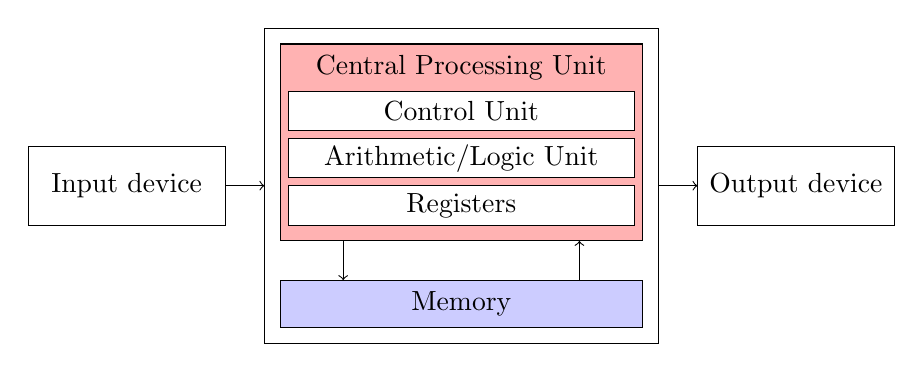
\begin{tikzpicture}
\draw (3,0) rectangle (8,4);
\draw (3.2,1.3) [fill=red!30] rectangle (7.8,3.8);
\node at (5.5,3.5) {Central Processing Unit};

\draw (3.3,1.5) [fill=white] rectangle (7.7,2.) node[pos=.5] {Registers};
\draw (3.3,2.1) [fill=white] rectangle (7.7,2.6) node[pos=.5] {Arithmetic/Logic Unit};
\draw (3.3,2.7) [fill=white] rectangle (7.7,3.2) node[pos=.5] {Control Unit};

\draw (0,1.5) rectangle (2.5,2.5) node[pos=.5] {Input device};
\draw (8.5,1.5) rectangle (11,2.5) node[pos=.5] {Output device};
\draw [->] (2.5,2) -- (3,2);
\draw [->] (8,2) -- (8.5,2);

\draw (3.2,.2) [fill=blue!20] rectangle (7.8,.8) node[pos=.5] {Memory};
\draw [->] (4,1.3) -- (4,.8);
\draw [->] (7,.8) -- (7,1.3);
\end{tikzpicture}
\caption{Von Neumann model}
\label{fig:1_HPC:von_neumann_model}
\end{figure}

John Von Neumann published its \textit{First Draft of a Report on the EDVAC}~\cite{von1993first} in 1945. 
Extracted from this work, the model know as the Von Neumann model or more generally Von Neumann Machine appears. 
The model is presented on figure~\ref{fig:1_HPC:von_neumann_model}.

On that figure we identify three parts, the input and output devices and in the middle the computational device itself. 
\paragraph{Input/Output devices}
The input and output devices are used to store in a read/write way data. 
They can be represented as hard drives, solid state drives, monitors, printers or even mouse and keyboard.
The input and output devices can also be the same, reading and writing in the same area.\\

Inside the computational device we find the memory, for the most common nowadays architectures it can be considered as a Random Access Memory (RAM). 
Several kind of memory exists and will be discussed later. 

\paragraph{Central Processing Unit}
The Central Processing Unit, CPU, is composed of several elements in this model. 
On one hand, the \textit{Arithmetic and Logic Unit}, ALU, which takes as input one or two values and apply an operation on those data. 
They can be either logics with operations such as AND, OR, XOR, etc. or arithmetics with operations such as ADD, MUL, SUB, etc. 
Of course those operations are way more complex on modern CPUs. 
On the other hand, we find the \textit{Control Unit}, CU, which control the data carriage to the ALU from the memory and the operation to be perform on data.
It is also the part that takes care of the Program Counter (PC), the address of the next instruction in the program. 
We can also identify the Register section which represent data location used for both ALU and CU to store temporary results, the current instruction address, etc. 
Some representation may vary, the Registers can be represented directly inside the ALU or the CU. 
\paragraph{Buses}
The links between those elements are called Buses and can be separated between data buses, control buses and addresses buses.
They will have a huge importance for the first machine optimization, growing the size of the buses from 2, 8, 16 to nowadays 32 and 64.\\

The usual processing flow on such an architecture can be summarized as a loop: 
\begin{itemize}[noitemsep,nolistsep]
\item[-] Fetch instruction at current PC from memory;
\item[-] Decode instruction using the Instruction Set Architecture (ISA). Known ISA are Reduce Instruction Set Computer architecture (RISC) and Complex Instruction Set Computer architecture (CISC);
\item[-] Evaluate operand(s) address(es);
\item[-] Fetch operand(s) from memory;
\item[-] Execute operation(s), with some instructions sets and new architectures several similar operations can be processed in the same clock time;
\item[-] Store results, increase PC.\\
\end{itemize}

Every devices or machines we describe in the next chapter have this architecture as a basis. 
One will consider execution models and architecture models to characterize HPC architectures.

\section{Flynn taxonomy and execution models}
\index{Flynn taxonomy}
The Von Neumann model gives us a generic idea of how a computational unit is fashioned. 
The constant demand in more powerful computers required the scientists to find more way to provide this computational power.
In 2001, IBM proposed the first multi-core processor on the same die, the Power4 with its 2 cores.
This evolution required new paradigms.
A right characterization is then essential to be able to target the right architecture for the right purpose. 
The Flynn taxonomy presents a hierarchical organization of computation machines and executions models.

\begin{table}
\centering
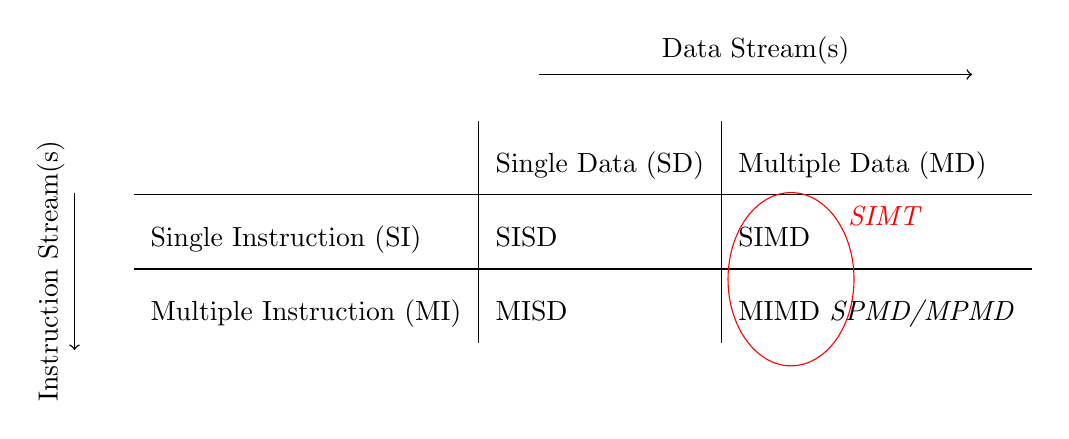
\begin{tikzpicture}
\node (table) {\arraycolsep=1.4pt\def\arraystretch{2.2}
\begin{tabular}{l | l | l}
 & Single Data (SD) & Multiple Data (MD) \\
 \hline 
Single Instruction (SI) & SISD & SIMD \\
\hline 
Multiple Instruction (MI) & MISD & MIMD \textit{SPMD/MPMD} \\
\end{tabular}
};
\draw [->,line width=.5pt] (-0.5,2) -- (5,2) node[midway, above] {Data Stream(s)};
\draw [->,line width=.5pt] (-6.4,0.5) -- (-6.4,-1.5) node[rotate=180,sloped, midway, above] {Instruction Stream(s)};
\draw [red] (2.7,-.6) ellipse (.8cm and 1.1cm) node[xshift=1.2cm,yshift=.8cm] {\textit{SIMT}};
%\draw[decoration={brace,raise=5pt},line width=1pt,decorate]
%  (5,0.4) -- node[right=6pt,yshift=5pt] {\textit{SIMT}} (5,-1.5);
\end{tikzpicture}
\caption{Flynn taxonomy for execution models completed with SPMD and SIMT models}
\label{tab:1_HPC:taxonomy_flynn}
\end{table}

\begin{figure}
\resizebox {.24\columnwidth} {!} {
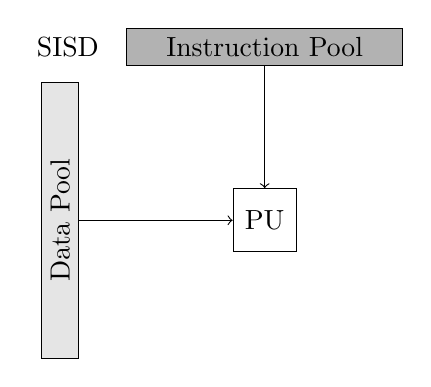
\begin{tikzpicture}
\draw (0.1,5.2) node {SISD}; 
\node (rect) at (2.6,5.2) [draw,minimum width=3.5cm,fill=black!30] (ip) {Instruction Pool};
\node (rect) at (0,3) [rotate=90,draw,minimum width=3.5cm,fill=black!10] (dp) {Data Pool};
\node (rect) at (2.6,3) [draw,minimum width=.8cm,minimum height=.8cm] (pu1) {PU};
\draw [->] (ip) -- (pu1);
\draw [->] (dp) -- (pu1);
\end{tikzpicture}
}
\resizebox {.24\columnwidth} {!} {
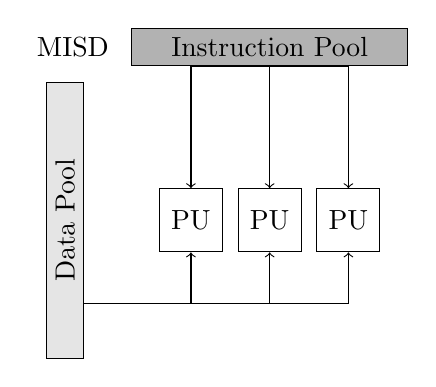
\begin{tikzpicture}
\draw (0.1,5.2) node {MISD}; 
\node (rect) at (2.6,5.2) [draw,minimum width=3.5cm,fill=black!30] (ip) {Instruction Pool};
\node (rect) at (0,3) [rotate=90,draw,minimum width=3.5cm,fill=black!10] (dp) {Data Pool};
\node (rect) at (1.6,3) [draw,minimum width=.8cm,minimum height=.8cm] (pu1) {PU};
\node (rect) at (3.6,3) [draw,minimum width=.8cm,minimum height=.8cm] (pu2) {PU};
\node (rect) at (2.6,3) [draw,minimum width=.8cm,minimum height=.8cm] (pu3) {PU};

\draw[<-] (pu1.north) |-  (ip.south); 
\draw[<-] (pu2.north) |-  (ip.south);
\draw[<-] (pu3.north) |-  (ip.south);

\draw[<-]  (pu1.south) |- ([yshift=-30pt]dp.south);
\draw[<-]  (pu2.south) |- ([yshift=-30pt]dp.south);
\draw[<-]  (pu3.south) |- ([yshift=-30pt]dp.south);

\end{tikzpicture}
}
\resizebox {.24\columnwidth} {!} {
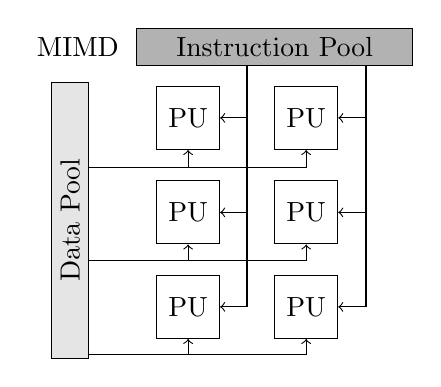
\begin{tikzpicture}
\draw (0.1,5.2) node {MIMD}; 
\node (rect) at (2.6,5.2) [draw,minimum width=3.5cm,fill=black!30] (ip) {Instruction Pool};
\node (rect) at (0,3) [rotate=90,draw,minimum width=3.5cm,fill=black!10] (dp) {Data Pool};
\node (rect) at (1.5,4.3) [draw,minimum width=.8cm,minimum height=.8cm] (pu1) {PU};
\node (rect) at (1.5,3.1) [draw,minimum width=.8cm,minimum height=.8cm] (pu2) {PU};
\node (rect) at (1.5,1.9) [draw,minimum width=.8cm,minimum height=.8cm] (pu3) {PU};
\node (rect) at (3,4.3) [draw,minimum width=.8cm,minimum height=.8cm] (pu4) {PU};
\node (rect) at (3,3.1) [draw,minimum width=.8cm,minimum height=.8cm] (pu5) {PU};
\node (rect) at (3,1.9) [draw,minimum width=.8cm,minimum height=.8cm] (pu6) {PU};

\draw[<-]  (pu1.south) |- ([yshift=19pt]dp.south);
\draw[<-]  (pu4.south) |- ([yshift=19pt]dp.south);

\draw[<-]  (pu2.south) |- ([yshift=-14.5pt]dp.south);
\draw[<-]  (pu5.south) |- ([yshift=-14.5pt]dp.south);

\draw[<-]  (pu3.south) |- ([yshift=-48.5pt]dp.south);
\draw[<-]  (pu6.south) |- ([yshift=-48.5pt]dp.south);

\draw[->] ([xshift=-10pt]ip.south) |- (pu1.east);
\draw[->] ([xshift=-10pt]ip.south) |- (pu2.east);
\draw[->] ([xshift=-10pt]ip.south) |- (pu3.east);

\draw[->] ([xshift=33pt]ip.south) |- (pu4.east);
\draw[->] ([xshift=33pt]ip.south) |- (pu5.east);
\draw[->] ([xshift=33pt]ip.south) |- (pu6.east);

%\draw[<-]  (pu2.south) |- ([yshift=-30pt]dp.south);
%\draw[<-]  (pu3.south) |- ([yshift=-30pt]dp.south);

%\draw [->] (ip) -- (pu1);
%\draw [->] (dp) -- (pu1);
\end{tikzpicture}
}
\resizebox {.24\columnwidth} {!} {
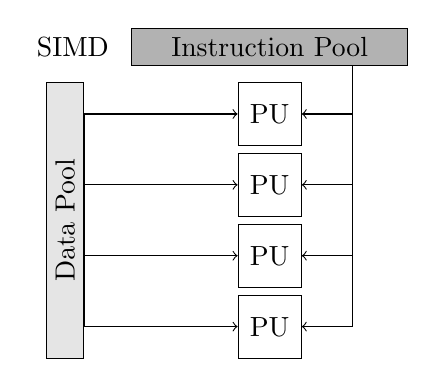
\begin{tikzpicture}
\draw (0.1,5.2) node {SIMD}; 
\node (rect) at (2.6,5.2) [draw,minimum width=3.5cm,fill=black!30] (ip) {Instruction Pool};
\node (rect) at (0,3) [rotate=90,draw,minimum width=3.5cm,fill=black!10] (dp) {Data Pool};
\node (rect) at (2.6,4.35) [draw,minimum width=.8cm,minimum height=.8cm] (pu1) {PU};
\node (rect) at (2.6,3.45) [draw,minimum width=.8cm,minimum height=.8cm] (pu2) {PU};
\node (rect) at (2.6,2.55) [draw,minimum width=.8cm,minimum height=.8cm] (pu3) {PU};
\node (rect) at (2.6,1.65) [draw,minimum width=.8cm,minimum height=.8cm] (pu4) {PU};
%\draw [->] ([yshift=2.35cm]dp) -- (pu1);
\draw[->] (dp.south) |- (pu1.west);
\draw[->] (dp.south) |- (pu2.west);
\draw[->] (dp.south) |- (pu3.west);
\draw[->] (dp.south) |- (pu4.west);

\draw[->] ([xshift=30pt]ip.south) |- (pu4.east);
\draw[->] ([xshift=30pt]ip.south) |- (pu3.east);
\draw[->] ([xshift=30pt]ip.south) |- (pu2.east);
\draw[->] ([xshift=30pt]ip.south) |- (pu1.east);
%\draw[arrow] (Small2B.north)--(Small2B|-Big2.south);s
%\draw [->] (dp) -- (pu1);
\end{tikzpicture}
}
\caption{Flynn taxonomy schematic representation of execution models}
\label{fig:1_HPC:flynn_taxonomy}
\end{figure}

In this classification~\cite{flynn1972some} from 1972, Michael J. Flynn presents the SISD, MISD, MIMD, and SIMD models represented on in table~\ref{tab:1_HPC:taxonomy_flynn} and figure~\ref{fig:1_HPC:flynn_taxonomy}.
Every of those execution model correspond to a specific machine and function.

\subsection{Single Instruction, Single Data: SISD}
This is the model corresponding to a single core CPU like in the Von Neumann model. 
This sequential model takes one instruction, operates on one data and the result is then store and the process continues over. 
SISD is important to consider as a reference computational time and will be considered in the next part for Amdahl's and Gustafson's laws.

\subsection{Multiple Instructions, Single Data: MISD}
This model can correspond to a pipelined computer.
Different operations are applied to the datum, which is transfered to the next computational unit and so on. 
This is the least common execution model.


\subsection{Multiple Instructions, Multiple Data: MIMD}
Every element executes its own instructions on its own data set. 
This can represent the behavior of a processor using several cores, threads or even the different nodes of a supercomputer cluster. 
Two subcategories can be identified in MIMD.

\subsubsection{SPMD}
The Single Program Multiple Data model, SPMD, is the most famous parallelism way for HPC purpose: each process execute the same program. 
At opposite to SIMD the programs are the same but does not share the same instruction counter. 
This model was proposed for the first time in \cite{darema1988single} in 1988 using Fortran.
This is the common approach working with runtime like MPI. 
The programs are the same and the execution similar but based on their ID the processes will target different data. 

\subsubsection{MPMD}
The Multiple Program Multiple Data model is also know for HPC. 
Generally with a separation between a main program generating data for sub-programs. 
This is the model on which we work in part II regarding the Langford problem resolution using split of the resolution tree.

\subsection{Single Instruction, Multiple Data: SIMD}
This is the execution model corresponding to a many-core architecture like a GPU. 
SIMD can be extended from 2 to 16 elements for classical CPUs to hundreds and even thousands of core for GPGPUs. 
In the same clock, the same operation is executed on every process on different data. 
The best example stay the work on matrices like a stencil, same instruction executed on every element of the matrix. 

\subsection{SIMT}
\index{SIMT}
We can also find another characterization to describe the new GPUs architecture: Single Instruction, Multiple Threads. 
This appears in one of NVIDIA's company paper~\cite{lindholm2008nvidia}. 
This model describes a combination of MIMD and SIMD architectures, every block of threads is working with the same control processor on different data and every block can have its own instruction counter.  
This is the model we describe in part \ref{sec:CUDA} used for the \textit{warps} model in NVIDIA CUDA.

\section{Memory}
\label{sec:NORMA}
In addition of the execution model and parallelism the memory access patterns have a main role on performances especially in SIMD and MIMD. 
In this classification we identify three categories: UMA, NUMA and NoRMA for shared and distributed cases. 
This model have been pointed out in the Johnson's taxonomy\cite{johnson1988completing}.

%We can also find Error-Correcting Code, ECC, memory which implements a bunch of data correction algorithm to guaranty the validity of them when error is not allowed. 

%\todo{MCDRAM}
%\todo{3D memory}

\begin{figure}
\centering 
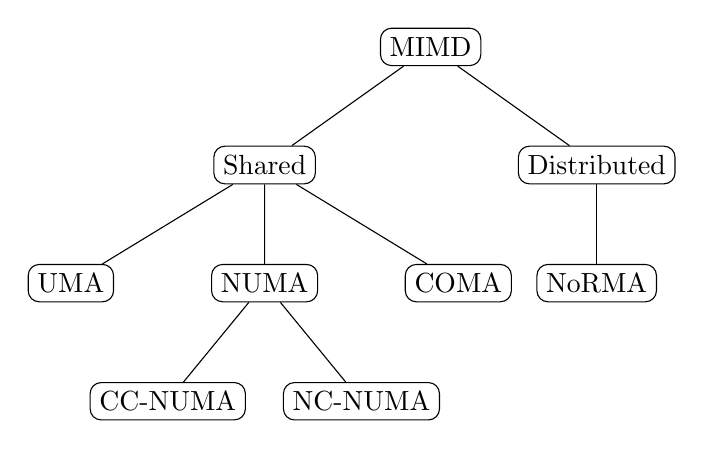
\begin{tikzpicture}[
   every node/.style = {
   level distance=1em,
   shape=rectangle, 
   rounded corners,
   draw, 
   align=center,
    top color=white%, 
   % bottom color=blue!20
   }]]
   \node {MIMD} [sibling distance=12em]
   child { node {Shared} [sibling distance=7em]
   child{node {UMA}} 
   child{node {NUMA}
   child{node {CC-NUMA}}
   child{node {NC-NUMA}}
   }
   child{node {COMA}}
   }
   child { node {Distributed}
   child { node {NoRMA}}
   };
\end{tikzpicture}
\caption{MIMD memory models}
\label{fig:1_HPC:mimd_memory_model}
\end{figure}

Those different types of memory for SIMD/MIMD model are summed up in figure~\ref{fig:1_HPC:mimd_memory_model}.

\subsection{Shared memory}
%In case of the SISD the memory access is just serial and no really rules needs to be set for its usage. 
When it comes to multi-threaded and multi-cores like MIMD or SIMD execution models several kind of memory models are possible. 
We give a description of the most common shared memories architectures. 

\hspace*{-2cm}
\begin{figure}
\centering 
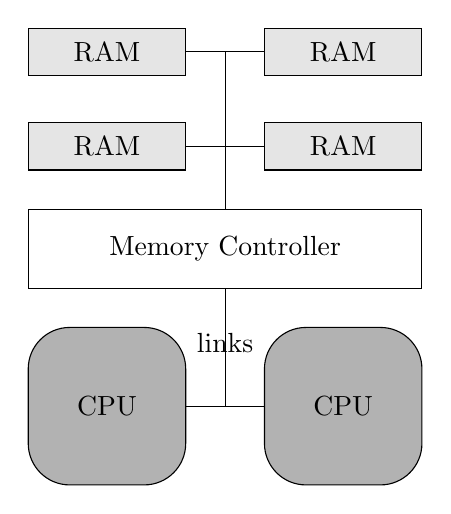
\begin{tikzpicture}
   \draw [rounded corners=15pt,fill=black!30] (0,0) rectangle (2,2) node[pos=.5] {CPU};
   \draw [rounded corners=15pt,fill=black!30] (3,0) rectangle (5,2) node[pos=.5] {CPU};

   \draw (0,2.5) rectangle (5,3.5) node[pos=.5] {Memory Controller};

   \draw (0,4) [fill=black!10] rectangle (2,4.6) node[pos=.5] {RAM};
   \draw (0,5.2) [fill=black!10] rectangle (2,5.8) node[pos=.5] {RAM};

   \draw (3,4) [fill=black!10] rectangle (5,4.6) node[pos=.5] {RAM};
   \draw (3,5.2) [fill=black!10] rectangle (5,5.8) node[pos=.5] {RAM};

   \draw [-] (2,1) -- (3,1);
   \draw [-] (2.5,1) -- (2.5,2.5);
	%\node at (2.5,2.2) {SDR, DDR, QDR};
	\node at (2.5,1.8) {links};

	\draw [-] (2.5,3.5) -- (2.5,5.5);
	\draw [-] (2,4.3) -- (3,4.3);
	\draw [-] (2,5.5) -- (3,5.5);
\end{tikzpicture}
\hspace{2cm}
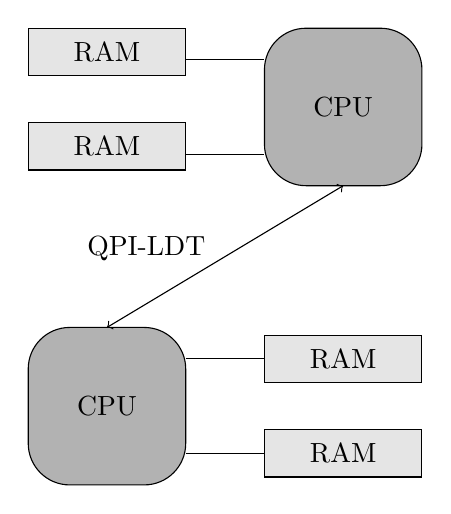
\begin{tikzpicture}
	\draw [rounded corners=15pt,fill=black!30] (0,0) rectangle (2,2) node[pos=.5] {CPU};
	\draw (3,0.1) [fill=black!10] rectangle (5,0.7) node[pos=.5] {RAM};
	\draw (3,1.3) [fill=black!10] rectangle (5,1.9) node[pos=.5] {RAM};
	\draw [-] (2,0.4) -- (3,0.4);
	\draw [-] (2,1.6) -- (3,1.6);

	\draw [rounded corners=15pt,fill=black!30] (3,3.8) rectangle (5,5.8) node[pos=.5] {CPU};
	\draw (0,4) [fill=black!10] rectangle (2,4.6) node[pos=.5] {RAM};
	\draw (0,5.2) [fill=black!10] rectangle (2,5.8) node[pos=.5] {RAM};
	\draw [-] (2,4.2) -- (3,4.2);
	\draw [-] (2,5.4) -- (3,5.4);

	\draw [<->] (1,2) -- (4,3.8);
	\node at (1.5,3) {QPI-LDT};
\end{tikzpicture}
%\hspace{1cm}
%\begin{tikzpicture}
%	\draw [rounded corners=15pt] (1,0) rectangle (3,2) node[pos=.5] {CPU};
%	\draw [rounded corners=15pt] (1,3.8) rectangle (3,5.8) node[pos=.5] {CPU};
%
%	\draw (0,2.1) rectangle (2,2.8) node[pos=.5] {RAM};
%	\draw (0,3.2) rectangle (2,3.8) node[pos=.5] {RAM};
%	
%	\draw (3,2.2) rectangle (5,2.8) node[pos=.5] {RAM};
%	\draw (3,2.2) rectangle (5,3.8) node[pos=.5] {RAM};
%
%\end{tikzpicture}
\caption{UMA vs NUMA memory models}
\label{fig:1_HPC:UMA_NUMA}
\end{figure}

\subsubsection{UMA}
The Uniform Memory Access is a global memory shared by every threads or cores. 
In UMA every processor uses its own cache as local private memory. 
The addresses can be accessed directly by each processor which makes the access time ideal. 
The downside is that more processors require more buses and thus UMA is hardly scalable. 
The cache consistency problem also appears in this context and will be discussed in next part. 
Indeed, if a data is loaded in one processor cache and modified, this information need to be spread to the memory and maybe other processes cache. 

With the arising of accelerators like GPUs and their own memory, some constructors found ways to create UMA with heterogeneous memory. 
AMD creates the heterogeneous UMA, hUMA~\cite{rogers2013amd}, in 2013 allowing CPU and GPU to target the same memory area.

\subsubsection{NUMA}

In Non Unified Memory Access every processor have access to its own private memory but allows other processors to access those area though Lightning Data Transport, LDT or Quick Path Interconnect, QPI, for Intel architectures. 

As we mention for the UMA memory, even if the processors does not directly access to the memory cache coherency is important. 
Two methods are possible: on one hand, the most used is Cache-Coherent NUMA (CC-NUMA) were protocols are used to keep data coherency through the memory. On the other hand No Cache NUMA (NC-NUMA) forces the processes to avoid cache utilization and write results in main memory losing all the benefits of caching data. 

\subsubsection{COMA}
In Cache-Only Memory Accesses, the whole memory is see as a cache from every processes.
Attraction memory is setting up and will attract the data near the process that will use those data. 
This model is less commonly use and lead to, in best cases, same results as NUMA.

\subsection{Distributed memory}

The previous models are based on shared memory, in the case where the processes can access memory of their neighbors processes. 
In some cases, like supercomputers, it would be too heavy for processors to handle the requests of all the others through the network. 
Each process or node will then possess its own local memory, that can be share with local processes. 
Then, in order to access to other nodes memory, communications through the network have to be done and copied in local memory. 
This distributed memory is called No Remote Memory Access (NoRMA).

\section{Performances characterization in HPC}
In the previous parts we described the different executions models, characterizations and memory models for HPC. 
Based on those tools we need to be able to emphasis the performances of a computer and a cluster. 

The performance can be of several kind. 
It can first be define by the speed of the processor itself with the frequency defined in GHz. 
This information is not perfect because the ALU is not busy all the time due to memory accesses, communications or side effects. 
It can be used to estimate the highest computational power of a machine. 

\subsection{FLOPS}
The Floating point Operation Per Second considers the number of floating-point operation that the system will executes in a second. 
They are an unit of performance for computers. 
Higher FLOPS is better. 
This is also the scale used to consider supercomputers computational power. 
For a cluster we can compute the theoretical FLOPS (peak) based on the processor frequency in GHz with:
\begin{equation}
FLOPS_{cluster} = \#nodes \times \frac{\#sockets}{\#node} \times \frac{\#cores}{\#socket} \times \frac{\#GHz}{\#core} \times \frac{FLOPS}{cycle}
\end{equation}

On figure~\ref{tab:1_HPC:flops_year}, the scale of FLOPS and the year of the first world machine is presented.
The next milestone, the exascale, is expected to be reach near 2020.  

\begin{table}
\[\arraycolsep=1.4pt\def\arraystretch{2.2}
\begin{tabular}{| l | l | l || l | l | l |}
\hline
	%\rowstyle{\bfseries}
	\textbf{Name} & \textbf{FLOPS} & \textbf{Year} & \textbf{Name} & \textbf{FLOPS} & \textbf{Year} \\
	\hline
	\hline
	kiloFLOPS & $10^{3}$ & & petaFLOPS  & $10^{15}$ & 2005 \\ 
	\hline
	megaFLOPS & $10^{6}$ & & exaFLOPS   & $10^{18}$ & 2020 ? \\
	\hline
	gigaFLOPS & $10^{9}$ & $\approx$ 1980  & zettaFLOPS & $10^{21}$ & \\
	\hline
	teraFLOPS & $10^{12}$ & 1996 & yottaFLOPS & $10^{24}$ & \\
	\hline
	\end{tabular}
	\]
	\caption{Floating-point Operation per Second and years of reach in HPC.}
	\label{tab:1_HPC:flops_year}
\end{table}

FLOPS is the main way to represent a computer's performance but other ways exists like Instructions Per Seconds (IPS), Instructions per Cycle (IPC) or Operations Per Second (OPS).
Some benchmarks also provide their own metrics. 

\subsection{Power consumption}
Another way to consider machine performance is to estimate the number of operations regarding the power consumption. 
It can consider all the previous metrics like FLOPS, IPS, IPC or OPS. 
Benchmarks, like the GREEN500, consider the FLOPS delivered over the watts consumed. 
For nowadays architectures the many-cores architectures like GPUs seems to deliver the best FLOPS per watt ratio.

\subsection{Scalability}
The scalability express the way a program react to parallelism. 
When an algorithm is implemented on a serial machine and is ideal to solve a problem, one may consider to use it on more than one core, socket, node or even cluster. 
Indeed, one may expect less computation time, bigger problem or a combination of both while using more resources. 
This completely depend on the algorithm parallelization and is expressed through scalability. 
A scalable program will scale on as many processors as we give, whereas a poorly scalable one will give same of even worst results as the serial code.  
Scalability can be approach using speedup and efficiency.

\subsection{Speedup and efficiency}
The latency is the time required to complete a task in a program.
\index{latency} 
Lower latency is better. 

The speedup compare the latency of both sequential and parallel algorithm. 
In order to get relevant results, one may consider the best serial program against the best parallel implementation.

Considering $n$, the number of processes, and $n=1$ the sequential case with $T_n$ the execution time working on $n$ processes and $T_1$ working on one process, the sequential execution time. 
The speedup can be defined using the latency by the formula: 
\index{Speedup}
\begin{equation}
\text{speedup} = S_n =  \frac{T_1}{T_n}
\end{equation}

\begin{figure}
\centering 
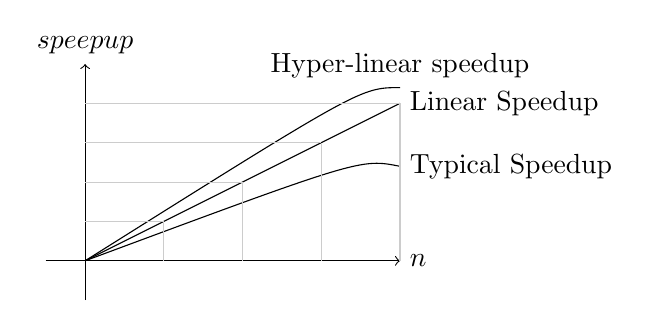
\begin{tikzpicture}
	\draw[->] (-.5,0) -- (4,0) node[right] {$n$};
	\draw[->] (0,-.5) -- (0,2.5) node[above] {$speepup$};
	\draw (0,0) -- (4,2) node[right] {\text{Linear Speedup}};
	\draw (0,0) .. controls (3.5,1.3) .. (4.,1.2) node[right] {\text{Typical Speedup}} ;
	\draw (0,0) .. controls (3.5,2.2) .. (4.,2.2) node[above] {\text{Hyper-linear speedup}} ;
   \draw[black!20] (1,0) -- (1,.5);
   \draw[black!20] (2,0) -- (2,1);
   \draw[black!20] (3,0) -- (3,1.5);
   \draw[black!20] (4,0) -- (4,2);
   \draw[black!20] (0,.5) -- (1,.5);
   \draw[black!20] (0,1) -- (2,1);
   \draw[black!20] (0,1.5) -- (3,1.5);
   \draw[black!20] (0,2) -- (4,2);
\end{tikzpicture}
\caption{Observed speedup: linear, typical and hyper-linear speedups}
\label{fig:1_HPC:speedup_obs}
\end{figure}

As shown on figure \ref{fig:1_HPC:speedup_obs} several kind of speedup can be observed. 
\paragraph{Linear}
The linear speedup usually represents the target for every program in HPC. 
Indeed, having the speedup growing exactly as the number of processors grows is the ideal case. 
Codes fall typical into two cases, typical and hyper-linear speedup. 
\paragraph{Typical speedup}
This represents the most common observed speedup. 
As the number of processors grows, the program face several of the HPC walls like communications wall or memory wall. 
The increasing number of computational power is reduced to the sequential part or lose time in communications/exchanges. 
\paragraph{Hyper-linear speedup}
In some cases we can observe an hyper-linear speedup, meaning that the results in parallel are even better than the ideal case. 
This can occur if the program can fit exactly in memory for less data on each processor or even fit perfectly for the cache utilization. 
The parallel algorithm can also be way more efficient than the sequential one.\\

In addition to speedup, the efficiency is defined by the speedup divided by the number of workers: 
\index{Efficiency}
\begin{equation}
\text{efficiency} = E_n = \frac{S_n}{n} = \frac{T_1}{nT_n}
\end{equation}
The efficiency, usually expressed in percent, represents the evolution of the code stability to growing number of processors. 
As the number of processes grows, a scalable application will keep an efficiency near 100\%.

\subsection{Amdahl's and Gustafson's law}
The Amdahl's and Gustafson's laws are ways to evaluate the maximal possible speedup for an application taking in account different characteristics. 

\subsubsection{Amdahl's law}
\index{Amdahl's law}
The Amdahl's law\cite{amdahl1967validity} is used to find the theoretical speedup in latency of a program.
We can separate a program into two parts, the one that can be execute in parallel and the one that is sequential. 
The law states that even if we reduce the parallel part using an infinity of processes the sequential part will reach 100\% of the total computation time. 

Extracted from the Amdahl paper the law can be written as: 

\begin{equation}
S_n = \frac{1}{Seq + \frac{Par}{n}}
\end{equation}

Where $Seq + Par = 1$ and $Seq$ and $Par$ respectively the sequential and parallel ratio of a program.
Here if we use up to $n=\inf$ processes, $S_n \leq \frac{1}{Seq}$ the sequential part of the code become the most time consuming. 

And the efficiency become:
\begin{equation}
E_n = \frac{1}{n\times Seq + Par}
\end{equation}

\begin{figure}
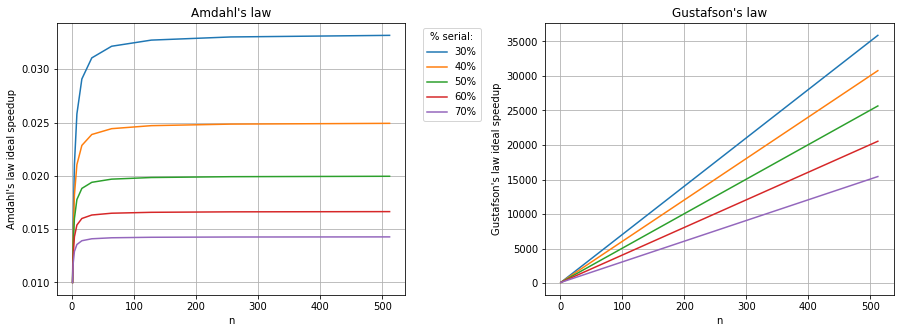
\includegraphics[width=\textwidth]{\locpath/figures/chap1/speedup_laws.png}
\caption{Theoretical speedup for Amdahl's (left) and Gustafson's (right) law}
\label{fig:1_HPC:speedup_laws}
\end{figure}

A representation of Amdahl's speedup is presented on Fig.~\ref{fig:1_HPC:speedup_laws} with varying percentage of serial part. 
The parallel part is like $Par = (100-Ser)\%$.

\subsubsection{Gustafson's law}
\index{Gustafson's law}
The Amdahl's law is focused on time with problem of the same size. 
John L. Gustafson's idea is that using more computational units, the problem size can grow accordingly. 
He considered a constant computation time with evolving problem, growing the size accordingly to the number of processes. 
Indeed the parallel part grows as the problem size do, reducing the percentage of the serial part for the overall resolution.

The speedup can now be estimated by:
\begin{equation}
S_n = Seq + Par \times n
\end{equation}

And the efficiency: 
\begin{equation}
E_n = \frac{Seq}{n} + Par
\end{equation}


Both Amdahl's and Gustafson's law are applicable and they represent two solution to check the speedup of our applications. 
The strong scaling\index{Strong scaling}, looking at how the computation time vary evolving only the number of processes, not the problem size. 
The weak scaling\index{Weak scaling}, at opposite to strong scaling we look how the computation time evolute varying the problem size keeping the same amount of work per processes. 

\section{Conclusions}

In this chapter we presented the different basic tools to be able to understand HPC: the Von Neumann model that is implemented in every nowadays architecture; the Flynn taxonomy that is in constant evolution with new paradigms like recent SIMT from NVIDIA. 
We also presented the memory types that will be use at different layers in our clusters, from node memory, CPU-GPGPU shared memory space to global fast shared memory. 
We finished by presenting the most important laws with Amdahl's and Gustafson's laws.
We introduced the concept of strong and weak scaling that will lead our tests through all the examples in Part II and Part III.

Those models have now to be confronted to the reality with hardware implementation and market reality, the vendors. 
The next part will introduce chronologically hardware and their optimization but always keeping a link with the models presented in this part. 
As there is always a gap between models and implementation we will have to find way to rank and characterize those architecture. 
This will be discuss in the last chapter. 
